% $Id: notes3.tex,v 1.11 2021/05/05 05:42:26 brandenb Exp $
%\documentclass{article}
\documentclass[twocolumn]{article}
\setlength{\textwidth}{160mm}
\setlength{\oddsidemargin}{-0mm}
\setlength{\textheight}{220mm}
\setlength{\topmargin}{-8mm}
\usepackage{graphicx,natbib,bm,url,color}
\graphicspath{{./fig/}{./png/}}
\thispagestyle{empty}
\input macros
\def\red{\textcolor{red}}
\def\blue{\textcolor{blue}}
\title{Maxwell equation with finite conductivity}
\author{Axel Brandenburg}
\date{\today}
\begin{document}
\maketitle

This text describes the implementation of
{\tt src/magnetic/maxwell.f90}.
It provides an exact solution, so time stepping
is only needed to interrupt the calculation
to provide diagnostic output in intermediate
intervals.

Assuming $\nab\cdot\AAA=\nab\cdot\EE=0$, we have
\begin{equation}
\dot{\AAA}=-\EE,\quad
\dot{\EE}=k^2\AAA-\sigma(\EE+\EMF).
\end{equation}
where $\EMF=\PPPP(\uu\times\BB)$ is the solenoidal part of
the electromagnetic force and $\PPPP$ is the projection operator.
\begin{equation}
\ddot{\AAA}+\sigma\dot{\AAA}+k^2\AAA=\sigma\EMF.
\end{equation}
The homogeneous part obeys the characteristic equation
\begin{equation}
\lambda^2+\lambda\sigma+k^2=0.
\end{equation}
Solution
\begin{equation}
\lambda_{1,2}=(-\sigma\pm D)/2
\end{equation}
where $D=\sqrt{\sigma^2-4k^2}$.
If $\sigma=0$, then $D=2\ii k$ and
$\lambda_{1,2}=\pm\ii k$.

\section{Solution}

From one time $t$ to the next $t+\delta t$, we assume that $\EMF=\const$.
We then make the following ansatz for each position in $\kk$ space:
\begin{equation}
\AAA=\AAA_1 e^{\lambda_1\delta t} + \AAA_2 e^{\lambda_2\delta t}
+(\sigma/k^2)\,\EMF,
\end{equation}
\begin{equation}
\EE=-\AAA_1 \lambda_1 e^{\lambda_1\delta t} - \AAA_2 \lambda_2 e^{\lambda_2\delta t}
\end{equation}
We define $\tilde{\AAA}=\AAA-(\sigma/k^2)\,\EMF$, so we have in matrix form
\begin{equation}
\pmatrix{\tilde{\AAA}\cr\EE}_{t+\delta t}=
\pmatrix{ 
e^{\lambda_1\delta t} & e^{\lambda_2\delta t} \cr
-\lambda_1 e^{\lambda_1\delta t} & -\lambda_2 e^{\lambda_2\delta t} }
\pmatrix{\AAA_1\cr\AAA_2}
\end{equation}
Initial condition
\begin{equation}
\pmatrix{\tilde{\AAA}\cr\EE}_t=
\pmatrix{ 
1 & 1 \cr
-\lambda_1 & -\lambda_2 }
\pmatrix{\AAA_1\cr\AAA_2},
\end{equation}
or
\begin{equation}
\pmatrix{\AAA_1\cr\AAA_2}
={1\over\lambda_1-\lambda_2}\pmatrix{ 
-\lambda_2 & -1 \cr
+\lambda_1 & +1 }
\pmatrix{\tilde{\AAA}\cr\EE}_t.
\end{equation}
So
\begin{equation}
\pmatrix{\tilde{\AAA}\cr\EE}_{t+\delta t}=
\pmatrix{c_A & s_A \cr s_E & c_E }=
\pmatrix{\tilde{\AAA}\cr\EE}_t.
\end{equation}
with
\begin{equation}
\pmatrix{c_A & s_A \cr s_E & c_E }=
\end{equation}
so, using $\lambda_1-\lambda_2=D$,
\begin{equation}
\pmatrix{ 
\nonumber
e^{\lambda_1\delta t} & e^{\lambda_2\delta t} \cr
-\lambda_1 e^{\lambda_1\delta t} & -\lambda_2 e^{\lambda_2\delta t} }
{1\over D}\pmatrix{ 
-\lambda_2 & -1 \cr
+\lambda_1 & +1 }
\nonumber
\end{equation}
or
\begin{equation}
{1\over D}\pmatrix{ 
\lambda_1 e^{\lambda_2\delta t} - \lambda_2 e^{\lambda_1\delta t} &
          e^{\lambda_2\delta t} -           e^{\lambda_1\delta t} \cr
\lambda_1 \lambda_2 (e^{\lambda_1\delta t} - e^{\lambda_2\delta t} ) &
\lambda_1 e^{\lambda_1\delta t} - \lambda_2 e^{\lambda_2\delta t} }
\end{equation}

For $\sigma=0$, this reduces to
\begin{equation}
{1\over2\ii k}\pmatrix{
\ii k e^{-\ii k\delta t} +\ii k e^{\ii k\delta t} &
      e^{-\ii k\delta t} -      e^{\ii k\delta t} \cr
\ii k (-\ii k) (e^{-\ii k\delta t} - e^{\ii k\delta t} ) &
\ii k e^{\ii k\delta t} +\ii k e^{-\ii k\delta t} }
\end{equation}
\begin{equation}
{1\over2}\pmatrix{
e^{-\ii k\delta t} + e^{\ii k\delta t} &
      (e^{-\ii k\delta t} -      e^{\ii k\delta t})/\ii k \cr
(-\ii k) (e^{-\ii k\delta t} - e^{\ii k\delta t} ) &
e^{\ii k\delta t} + e^{-\ii k\delta t} }
\end{equation}
\begin{equation}
=\pmatrix{
\cos k\delta t & -k^{-1}\sin k\delta t \cr
k \sin k\delta t & \cos k\delta t }
\end{equation}

\begin{figure}[b!]\begin{center}
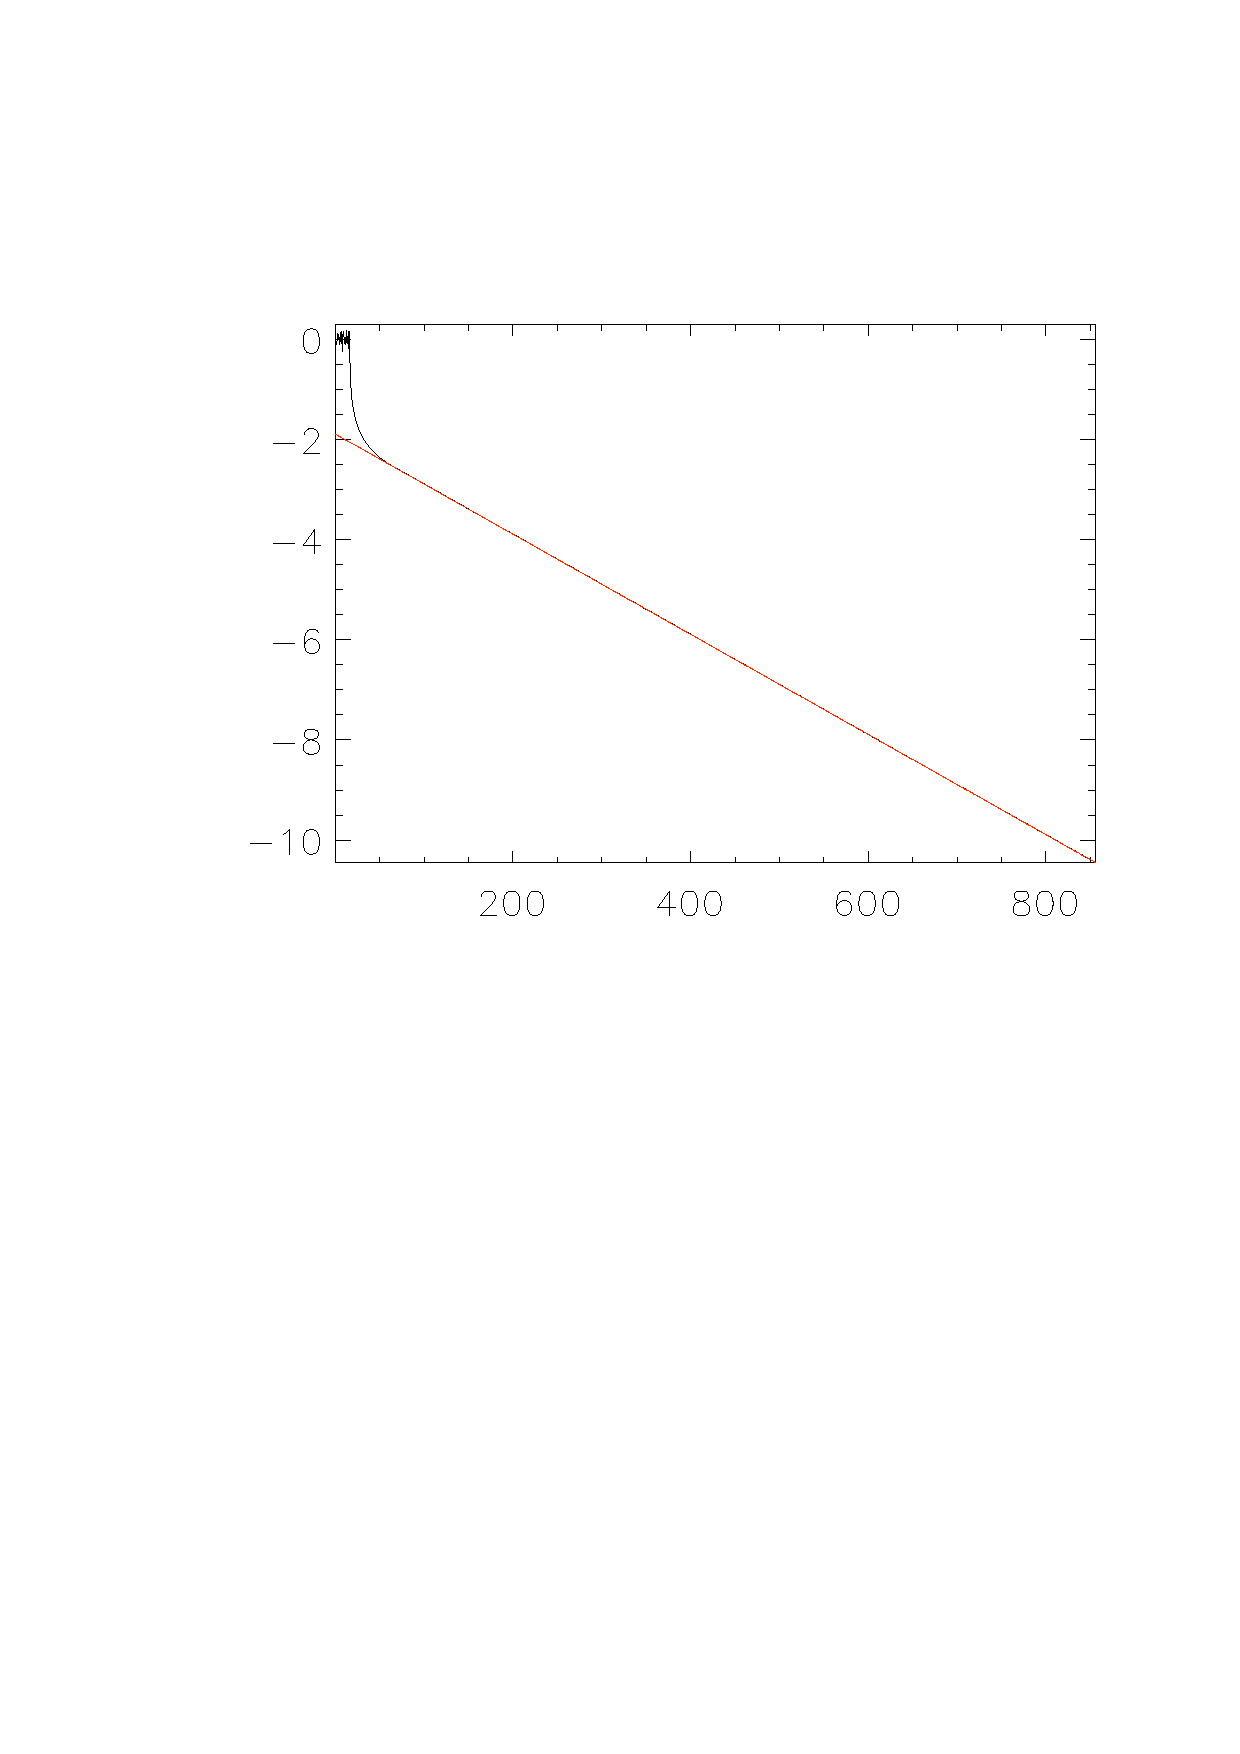
\includegraphics[width=\columnwidth]{pdecay}
\end{center}\caption[]{
Decay of $l=\ln\Brms$ for a linearly increasing conductivity.
}\label{pdecay}\end{figure}

\begin{figure}[b!]\begin{center}
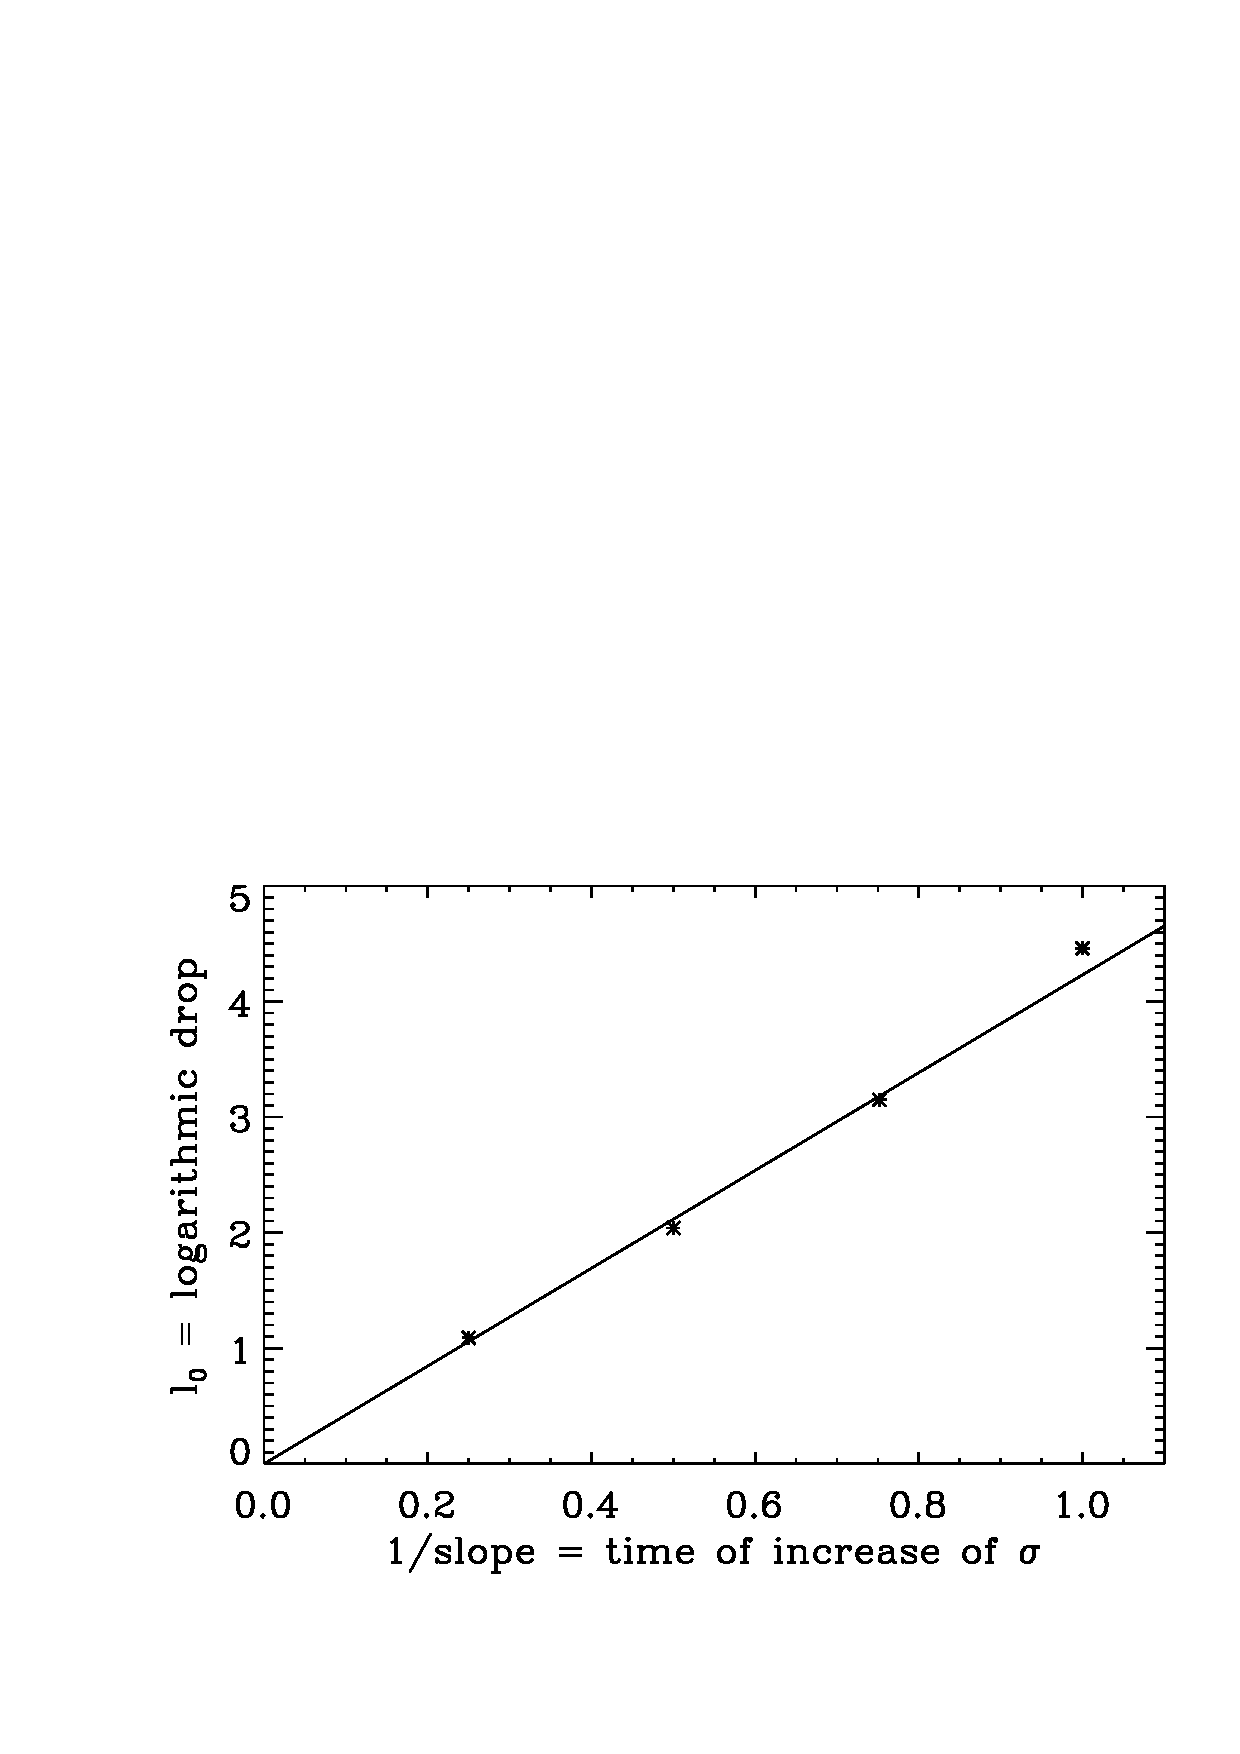
\includegraphics[width=\columnwidth]{plaw}
\end{center}\caption[]{
Decay of $l=\ln\Brms$ on the slope $s$
for a linearly increasing conductivity.
}\label{plaw}\end{figure}

\begin{figure}[b!]\begin{center}
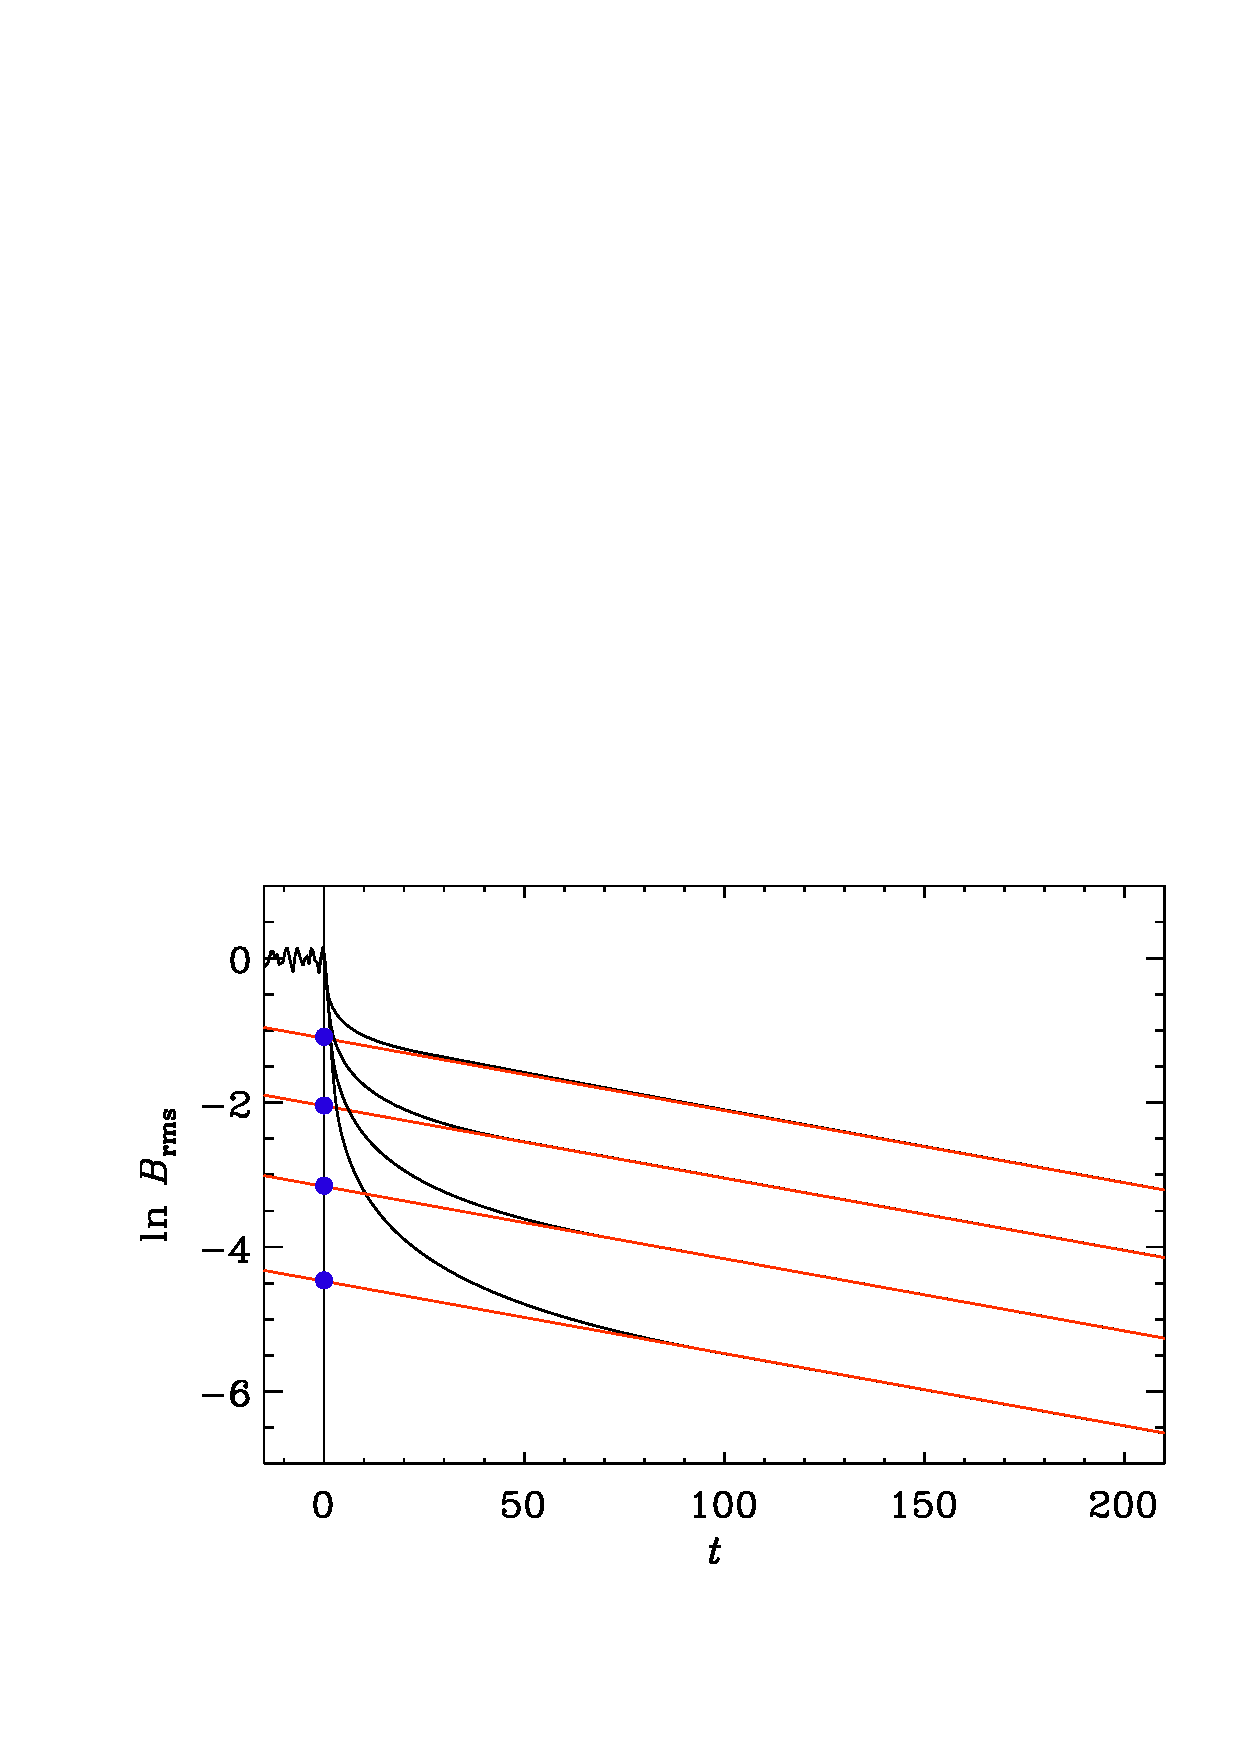
\includegraphics[width=\columnwidth]{pcomp_decay}
\end{center}\caption[]{
Decay of $l=\ln\Brms$ for a linearly increasing conductivity.
}\label{pcomp_decay}\end{figure}

In the limit $\sigma\to\infty$, we have $D=\sigma-2k^2/\sigma$, so
$\lambda_1=-k^2/\sigma$ and $\lambda_2=-\sigma$,
\begin{equation}
c_A\approx{1\over\sigma}\left(1+{2k^2\over\sigma^2}\right)
\left(-{k^2\over\sigma}e^{-\sigma\delta t}+\sigma e^{-k^2\delta t/\sigma}\right)
\end{equation}
or, expanding $e^{-k^2\delta t/\sigma}\approx1-k^2\delta t/\sigma$,
\begin{equation}
c_A\approx\left(1+{2k^2\over\sigma^2}\right)
\left(-{k^2\over\sigma^2}e^{-\sigma\delta t}+1-{k^2\over\sigma}\delta t \right)
\end{equation}
we have $c_A\approx1-\delta t \, k^2/\sigma$, and the matrix becomes
\begin{equation}
%\pmatrix{
%1+\delta t k^2/\sigma & (e^{-\sigma\delta t}-1)/\sigma \cr
%0 &  e^{-\sigma\delta t}}
\approx
\pmatrix{
1-\delta t \, k^2/\sigma & -\sigma^{-1} \cr
0 & e^{-\sigma\delta t} }
\end{equation}
Therefore,
\begin{equation}
\AAA_{\rm new}-{\sigma\over k^2}\EMF
=\left(1-\delta t {k^2\over\sigma}\right)\left(\AAA-{\sigma\over k^2}\EMF\right)
-{\EE\over\sigma}.
\end{equation}
so
\begin{equation}
\AAA_{\rm new}={\sigma\over k^2}\EMF
+\left(1-\delta t {k^2\over\sigma}\right)\left(\AAA-{\sigma\over k^2}\right)\EMF
-{\EE\over\sigma}.
\end{equation}
or
\begin{equation}
\AAA_{\rm new}={\sigma\over k^2}\EMF
+\left(1-\delta t {k^2\over\sigma}\right)\AAA
-\left(1-\delta t {k^2\over\sigma}\right){\sigma\over k^2}\EMF
-{\EE\over\sigma}.
\end{equation}
and therefore
\begin{equation}
\AAA_{\rm new}=
\left(1-\delta t \, {k^2\over\sigma}\right)\AAA
+\delta t \, \EMF
-{\EE\over\sigma}.
\end{equation}
Ignoring also the $-\EE/\sigma$ term, we have
\begin{equation}
{\AAA_{\rm new}-\AAA\over \delta t}=-{k^2\over\sigma}\AAA+\EMF
\end{equation}
so we recover, to first order,
\begin{equation}
{\partial\AAA\over\partial t}=-\eta k^2\AAA+\EMF,
\end{equation}
where $\eta=1/\sigma$ is the magnetic diffusivity.

\section{Conductivity changes}

Assume $\sigma=st$ after $t>t_0$ up to some maximum value $\sigma_2$.
At late times, $\Brms\propto\exp(-t k^2/\sigma$.
We extrapolate $l=l_0$ back to the time $t_0$ when $\sigma$ was still constant;
see \Fig{pdecay}.

\Fig{plaw} shows the dependence $l_0$ versus $1/s$.
There seems to be a linear relationship between $l_0$ and the
time of increase of $\sigma$.
\Fig{pcomp_decay} shows the decay of $l=\ln\Brms$ for a
linearly increasing conductivity with different time constants.

\section{Displacement as a correction}

\begin{equation}
\dot{\AAA}=-\EE,\quad
{1\over c^2}{\partial\EE\over\partial t}=k^2\AAA-\sigma(\EE+\EMF).
\end{equation}
Isolate $\EE$
\begin{equation}
\left(\sigma+{1\over c^2}{\partial\over\partial t}\right)\EE=k^2\AAA-\sigma\EMF.
\end{equation}
Divide by $\sigma$
\begin{equation}
\left(1+{\eta\over c^2}{\partial\over\partial t}\right)\EE=-(\EMF+\eta\nabla^2\AAA).
\end{equation}
\begin{equation}
\left(1+{\eta\over c^2\delta t}\right)\EE=
{\eta\over c^2\delta t}\EE_{\rm old}
-(\EMF+\eta\nabla^2\AAA).
\label{FirstOrder}
\end{equation}
In the limit $\eta\to0$, we recover
\begin{equation}
\EE=-(\EMF+\eta\nabla^2\AAA).
\end{equation}
In the limit $\eta\to\infty$, we recover
\begin{equation}
{\eta\over c^2\delta t}\EE=
{\eta\over c^2\delta t}\EE_{\rm old}
-\eta\nabla^2\AAA.
\end{equation}
\Eq{FirstOrder} in terms of $\sigma$
\begin{equation}
\left(1+{1\over c^2\sigma\delta t}\right)\EE=
{1\over c^2\sigma\delta t}\EE_{\rm old}
-(\EMF+\eta\nabla^2\AAA).
\end{equation}
Define $\epsilon=(c^2\sigma\delta t)^{-1}$, then
\begin{equation}
\EE={\epsilon\over1+\epsilon}\EE_{\rm old}
-{1\over1+\epsilon}(\EMF+\eta\nabla^2\AAA).
\end{equation}
Limit $\epsilon\to0$
\begin{equation}
\EE=-(\EMF+\eta\nabla^2\AAA).
\end{equation}
Limit $\epsilon\to\infty$, usimg $\epsilon^{-1}=c^2\sigma\delta t$
\begin{equation}
\EE=\EE_{\rm old}
-c^2\sigma\delta t(\EMF+\eta\nabla^2\AAA).
\end{equation}


%r e f
%\begin{thebibliography}{}

%\bibitem[Biskamp \& M\"uller(1999)]{BM99}
%Biskamp, D., \& M\"uller, W.-C.\yprl{1999}{83}{2195}

%\end{thebibliography}

\vfill\bigskip\noindent\tiny\begin{verbatim}
$Header: /var/cvs/brandenb/tex/GW/inflation/notes3.tex,v 1.11 2021/05/05 05:42:26 brandenb Exp $
\end{verbatim}

\end{document}
